\documentclass[3p, authoryear]{elsarticle} %review=doublespace preprint=single 5p=2 column
%%% Begin My package additions %%%%%%%%%%%%%%%%%%%
\usepackage[hyphens]{url}

  \journal{Submitted to Transportation Research Part C: Emerging Technologies} % Sets Journal name


\usepackage{lineno} % add
\providecommand{\tightlist}{%
  \setlength{\itemsep}{0pt}\setlength{\parskip}{0pt}}

\usepackage{graphicx}
\usepackage{booktabs} % book-quality tables
%%%%%%%%%%%%%%%% end my additions to header

\usepackage[T1]{fontenc}
\usepackage{lmodern}
\usepackage{amssymb,amsmath}
\usepackage{ifxetex,ifluatex}
\usepackage{fixltx2e} % provides \textsubscript
% use upquote if available, for straight quotes in verbatim environments
\IfFileExists{upquote.sty}{\usepackage{upquote}}{}
\ifnum 0\ifxetex 1\fi\ifluatex 1\fi=0 % if pdftex
  \usepackage[utf8]{inputenc}
\else % if luatex or xelatex
  \usepackage{fontspec}
  \ifxetex
    \usepackage{xltxtra,xunicode}
  \fi
  \defaultfontfeatures{Mapping=tex-text,Scale=MatchLowercase}
  \newcommand{\euro}{€}
\fi
% use microtype if available
\IfFileExists{microtype.sty}{\usepackage{microtype}}{}
\usepackage{natbib}
\bibliographystyle{plainnat}
\usepackage{longtable}
\usepackage{graphicx}
% We will generate all images so they have a width \maxwidth. This means
% that they will get their normal width if they fit onto the page, but
% are scaled down if they would overflow the margins.
\makeatletter
\def\maxwidth{\ifdim\Gin@nat@width>\linewidth\linewidth
\else\Gin@nat@width\fi}
\makeatother
\let\Oldincludegraphics\includegraphics
\renewcommand{\includegraphics}[1]{\Oldincludegraphics[width=\maxwidth]{#1}}
\ifxetex
  \usepackage[setpagesize=false, % page size defined by xetex
              unicode=false, % unicode breaks when used with xetex
              xetex]{hyperref}
\else
  \usepackage[unicode=true]{hyperref}
\fi
\hypersetup{breaklinks=true,
            bookmarks=true,
            pdfauthor={},
            pdftitle={If you build it who will come? Equity analysis of park system changes using passive origin-destination data},
            colorlinks=false,
            urlcolor=blue,
            linkcolor=magenta,
            pdfborder={0 0 0}}
\urlstyle{same}  % don't use monospace font for urls

\setcounter{secnumdepth}{5}
% Pandoc toggle for numbering sections (defaults to be off)


% Pandoc header
\usepackage{booktabs}
\usepackage{longtable}
\usepackage{array}
\usepackage{multirow}
\usepackage{wrapfig}
\usepackage{float}
\usepackage{colortbl}
\usepackage{pdflscape}
\usepackage{tabu}
\usepackage{threeparttable}
\usepackage{threeparttablex}
\usepackage[normalem]{ulem}
\usepackage{makecell}
\usepackage{xcolor}



\begin{document}
\begin{frontmatter}

  \title{If you build it who will come? Equity analysis of park system changes using passive origin-destination data}
    \author[BYU]{Gregory Macfarlane\corref{1}}
   \ead{gregmacfarlane@byu.edu} 
    \author[StreetLight]{Teresa Tapia}
   \ead{teresa.tapia@streetlightdata.com} 
    \author[Harvard]{Carole Turley-Voulgaris}
   \ead{cvoulgaris@gsd.harvard.edu} 
      \address[BYU]{Brigham Young University, Civil and Environmental Engineering Department, 430 Engineering Building, Provo, Utah 84602}
    \address[Harvard]{Harvard Graduate School of Design, 48 Quincy St, Cambridge, Massachussetts 02138}
    \address[StreetLight]{StreetLight Data, Inc., San Francisco, California}
      \cortext[1]{Corresponding Author}
  
  \begin{abstract}
  Parks provide important benefits to those who live near them, in the form of improved property values, health outcomes, etc.; nevertheless, measuring and understanding who lives near a park is an open research question. In particular, it is not well understood which park individuals will choose to use when given a choice among a set of nearby parks of varying sizes and at varying distances from their home. In this paper we present a park activity location choice model estimated from a passive origin-destination dataset --- supplied by StreetLight Data, Inc.~--- representing trips to parks and green spaces in Alameda County, California. The estimated model parameters reveal heterogeneous preferences for park size and willingness-to-travel across block-group level socioeconomic segmentation: Specifically, high-income block groups appear more positively attracted to larger parks, and block groups with a high proportion of ethnic minority individuals are more likely to select nearby parks. The findings have importance for understanding recreational access among different populations, and the methodology more generally supplies a potential template for using passive data products within travel modeling.
  \end{abstract}
   \begin{keyword} Accessibility Passive Data Location Choice\end{keyword}
 \end{frontmatter}

\hypertarget{intro}{%
\section{Introduction}\label{intro}}

Parks and other green spaces generate immense value for the public who are able
to access them. The \citet{CityParksAlliance} categorizes the observed benefits of
urban parks as encouraging active lifestyles \citep{Bancroft2015}, contributing to
local economies, aiding in stormwater management and flood mitigation,
improving local air quality, increasing community engagement \citep{Madzia2018}, and
enhancing public equity.

Nevertheless, understanding and quantifying these benefits depends in many
cases on identifying who lives near the parks and is therefore able to access
them. Many previous studies \citep[e.g.,][]{Richardson2012} rely on comparison of total
greenspace across metropolitan areas; this methodology may not adequately
control for city-level fixed effects and it may ignore the potentially
inequitable distribution of park space within a region. Studies focusing on
access within metropolitan areas typically assume that people living within a
certain distance or travel time threshold have access to a park, or examine the
quantity of park space within one's own arbitrarily defined ``neighborhood''
\citep[Stark2014]{Mitchell2008}. But these methods do not account for the fact that
some people will travel to other parks to perform recreational activities. A
more holistic measure that continuously measures access across multiple
preference dimensions is desirable.

An appealing solution would be to examine and model the activity location
choices of park users. Such a model would help researchers understand how
individuals of different backgrounds and preferences value different park
amenities. Further, the logsums of a location choice model provide a continuous
measure of accessibility that explicitly accounts for such variation
\citep{DeJong2007}. Unfortunately, park choice models of this form are rare in the
literature. Travel demand models built for infrastructure forecasting are a
common way to generate such accessibility logsums, but these models group many
different kinds of social and recreational trips together \citep{nchrp716}. Further,
the attraction term for such trip purposes is commonly a function of the retail
or service employment or the number of households at the destination; a typical
park or green space has neither employees nor residents. Finally, many regional
household travel surveys are oriented towards an average weekday travel
pattern, and many park trips occur irregularly or on weekends.

In this paper we present a park destination choice model where individuals
living in Alameda County, California choose among parks in the same county. The
individuals are constructed from passive data that was derived from mobile
devices and processed using algorithms developed by StreetLight Data, Inc.~The
origin location points are inferred residence block groups for unique devices
and the destination points are geofenced polygons representing green and open
spaces. The individuals' choice of park location is conditioned on the distance
from the block group to the parks in the choice set as well as the size of each
park; market segmentation allows for heterogeneous responses between ethnic
groups and income strata.

The paper proceeds in the following manner: A discussion of prior attempts to
study park choice and employ passive origin-destination data in the literature
is given directly. The Methodology section presents the data gathering and
cleaning efforts as well as the econometric location choice model. The Results
section presents the estimated model coefficients and a discussion of the
findings, as well as a model validation exercise. After presenting limitations
and associated avenues for future research, a final Conclusions section
outlines the contributions of this study for recreational trip modeling and
location choice modeling more generally.

\hypertarget{literature}{%
\section{Literature}\label{literature}}

\hypertarget{defining-and-measuring-park-accessibility}{%
\subsection{Defining and measuring park accessibility}\label{defining-and-measuring-park-accessibility}}

\citet{Handy1997} identify three broad types of accessibility measures: cumulative
opportunity measures, gravity-based measures, and utility-based measures.
\citet{GEURS2004127} classify cumulative opportunity and gravity-based measures into
a single category that they refer to as location-based measures. Researchers
have applied versions of location-based measures and, to a lesser degree,
utility-based measures to quantify park accessibility

\hypertarget{location-based-measures-of-park-accessibility}{%
\subsubsection{Location-based measures of park accessibility}\label{location-based-measures-of-park-accessibility}}

Cumulative opportunity measures are calculated by counting the number of origins
or destinations within a threshold travel cost of a location (where cost might
be some combination of distance, travel time, and/or monetary cost of travel). A
strength of cumulative opportunity measures lies in their simplicity and
intuitive interpretation. However, they may be too simple, especially with
regard to trip costs near the threshold. An example of a cumulative opportunity
measure might be the number of parks within a ten-minute walk of a person's
home, or the number of households living within ten minutes of a park. This
measure would imply that a household living immediately adjacent to a park has
the same access to it as one that lives nine minutes away, but that a household
living eleven minutes away has no access to it.

ParkScore \citep{parkscore2019}, developed by the Trust for Public Land, is a popular
measure of park accessibility that starts from a cumulative opportunity measure
(the share of the population that resides within a 10-minute walk of a green
space) and adjusts this value based on the total city green space, investment,
and amenities weighted against the socioeconomic characteristics of the
population outside of the 10-minute walk threshold. The resulting score is a
convenient quantitative tool in estimating the relative quality of green space
access across cities \citep{Rigolon2018}. It may be less useful at identifying the
comparative quality of access within a city, particularly since more than 95\% of
residents in many dense metropolitan areas like San Francisco and New York may
live within the binary 10-minute walk threshold {[}citation needed{]}. The Centers
for Disease Control and Prevention (CDC) has developed an ``Accessibility to
Parks Indicator'' along similar lines \citep{Ussery2016}, calculating the share of the
population living within a half-mile of a park for each county in the U.S.

Gravity-based accessibility measures take a similar approach to cumulative
opportunity measures, but theoretically include all possible destinations and
weight them according to the travel cost that they impose, based on an impedance
function. Cumulative opportunity measures may be considered a special case of
gravity-based measures, where the impedance function takes the form of a binary
step function that equals zero after a cutoff travel cost (which is why
\citet{GEURS2004127} classify them both as location-based). The inverse square function
is a common form of impedance function for gravity-based accessibility measures.

A major advantage of gravity-based accessibility measures lies in their
consistency with travel behavior theory: Gravity-based measures have their roots
in the trip-distribution step of the traditional four-step travel demand
forecasting method, where trips originating in a particular zone are distributed
among destination zones, proportionate to each zone's gravity-based
accessibility. Urban scholars have used gravity-based measures to explore the
spatial distribution of park access across Tainan City, Taiwan
\citep{chang2011exploring} and to estimate the relationship between park access and
housing prices in Shenzhen, China \citep{wu2017spatial}.

Some scholars have used location-based measures of park accessibility to
evaluate equity in park access. \citet{chang2011exploring} use a gravity-based measure
to determine that low-income neighborhoods have less access to parks than
higher-income neighborhoods in Tainan City, Taiwan. \citet{bruton2014disparities}
conduct a neighborhood-level analysis of park amenities in Greensboro, North
Carolina, and find that low-income neighborhoods tend to have parks with more
picnic areas, more trash cans, and fewer wooded areas, but they do not address
the question of the extent to which different populations might value these
different amenities. \citet{kabisch2014green} find that neighborhoods in Berlin with
high immigrant populations and older populations likewise had less access to
parks, and they pair these findings with survey results suggesting that these
disparities are not consistent with the preferences expressed by those
populations.

The question of whether uneven distribution of parks and park amenities might
reflect local preferences could be more appropriately addressed using
utility-based measures of park accessibility (as discussed below) and though
qualitative studies (as discussed in the following section).

\hypertarget{utility-based-measures-of-park-accessibility}{%
\subsubsection{Utility-based measures of park accessibility}\label{utility-based-measures-of-park-accessibility}}

While traditional four-step travel demand models distribute zonal trips based on
a gravity-based accessibility model, the travel demand modeling profession has
shifted more recently towards a destination choice framework that distributes
trips based on discrete-choice regression models. \citet{mcfadden1974measurement} first applied
discrete choice models to urban travel demand to predict mode choice, and
activity-based models apply them to all travel behavior choices, including to
select among alternative routes or alternative destinations \citep{de2011modelling}.
Though the application of random utility models to destination choice is not new
\citep[see][]{anas1983discrete}, the increasing availability of computing resources makes
estimating and applying discrete choice models on large alternative sets in a
practical context more feasible.

When applied to destination choice, discrete choice models estimate the
likelihood of selecting a particular destination among a set of alternatives
based on the relative attractiveness, or \emph{utility}, of each alternative. Utility
may be function of distance or travel time alone (in which case, a utility-based
accessibility measure might be quite similar to a location-based measure), but
it can also incorporate other destination characteristics that lead one
destination to be more highly-utilized than another. For a utility-based measure
of park accessibility, these might include park size or park amenities.

Destination-choice models have not commonly been used to measure park
accessibility, scholars have acknowledged that park accessibility metrics should
be linked with park use, since a park that has many visitors must by definition
be accessible to those visitors. \citet{McCormack2010} provide a comprehensive review
of this literature; it is sufficient here to note that most studies find park
use to depend on a complicated interplay between park size, maintenance,
facilities, and travel distance. Many of these attributes are incorporated into
ParkIndex \citep{Kaczynski2016}, which estimates the resident park use potential
within \(100 m^2\) grid cells, based on a household park use survey in Kansas
City.

The park use potential measured by ParkIndex is not dissimilar from a park trip
production potential, as used by transportation planners and engineers. Along
these lines, the question of park use is a destination choice problem, where
trip makers consider which park is most attractive to accomplish their
recreation activity. The Institute of Transportation Engineers (ITE) Trip
Generation Manual \citeyearpar{ite2019} contains trip attraction rates for public parks
that use the park acreage, number of picnic tables, employees, and other
variables as attraction terms. As with many land uses in Trip Generation, the
provided trip generation rates are based on a limited number of observational
samples \citep{shoup_truth_2003} and may not represent large-sample behavior
\citep{Millard-Ball2015}. Moreover, regression-based attraction rates isolated from
trip production and travel behavior ignore the geographical and behavioral
contexts in which people actually make trips to parks \citep{Barnard1987}: Though
more people may come to larger parks, planners cannot bring more people to a
park simply by increasing its size.

There are limited examples of researchers using a destination choice model to
predict recreation attractions. \citet{Kinnell2006} apply a choice model to a survey of
park visitors in New Jersey, and estimate the relative attractiveness of park
attributes including playgrounds, picnic areas, and park acreage weighed against
the travel disutility and the relative crime rate at the destination. In a
similar study, \citet{Meyerhoff2010} model the urban swimming location choice for a
surveyed sample. In both studies, the researchers were attempting to ascertain
which attributes of a recreation generated the most positive utility, and
therefore which attributes should be prioritized for improvement. These studies
have not to our knowledge been previously referenced in discussions of park
accessibility.

One obstacle to estimating discrete-choice models to estimate park choice has
been the lack of sufficiently detailed, trip-level data. The advent of
large-scale mobile networks and the seemingly perpetual association of unique
devices with unique users has given researchers a new opportunity to observe the
movements and activity location patterns for large subsets of the population
\citep{Naboulsi2016}. Such passively collected movement data --- sometimes referred
to as ``Big Data'' --- is a by-product of other systems including cellular call
data records \citep[e.g.,][]{Bolla2000, Calabrese2011}, probe GPS data \citep{Huang2015},
and more recently Location Based Services (LBS) \citep{Roll2019, Komanduri2017}. LBS
use a network of mobile applications that obtain the users' physical location. A
variety of commercial vendors repackage, clean, and scale these data to
population or traffic targets and sell origin-destination matrices to
researchers and practitioners at relatively low prices. \citet{Monz2019}, for example,
demonstrate how passive device data can be used to accurately estimate trips to
natural
recreation areas.

Passive origin-destination matrices are beginning to inform trip distribution
model development more directly as well. \citet{tf_idea} proposes one methodology,
where passive origin-destination matrices serve as a probabilistic sampling
frame for a simulated trip destination choice. \citet{Bernardin2018} employ a passive
origin-destination matrix as a shadow price reference in an activity-based
location choice model, iteratively adjusting the parameters of the choice
utilities to minimize the observed error between the matrix and the modeled
predictions. A similar method developed by \citet{Zhu2018} uses the passive dataset
directly, sampling 10,000 random trips from GPS traces of taxi trips in Shanghai
and estimating a destination choice model. Employing the passive data set in
this way provides the authors an opportunity to examine the choices of a large
sample of a small population (taxi passengers) as well as sufficient data to
estimate a ``constants-rich'' destination choice model with uniquely estimated
coefficients for each origin-destination pair. The \citet{Zhu2018} methodology suggests
that a similar approach should apply in other contexts, including park choice.
Applying these models to park choice allows us to not only predict potential
park use, but also determine which park characteristics are most valuable to
particular populations. The results of such an analysis offer an important
complement to existing qualitative and survey-based research on park use by
marginalized populations.

\hypertarget{sociodemographic-variation-in-park-utility}{%
\subsection{Sociodemographic variation in park utility}\label{sociodemographic-variation-in-park-utility}}

The idea that different racial, ethnic, or cultural groups have different
recreational styles, and might thus have different needs and preferences for
parks and open space, has been thoroughly discussed in the leisure studies
literature, and \citet{husbands1995ethnicity} offer a detailed review of that research
as of the mid-1990s. In general, explanations for racial and ethnic differences
in park use can be classified into two categories: those rooted in cultural and
lifestyle differences, and those rooted in discrimination and marginalization.

\citet{byrne2009nature} summarize literature in the former category, noting that
African Americans have been described as preferring more social,
sports-oriented spaces, relative to white people who prefer secluded natural
settings \citep{washburne1978black, hutchison1987ethnicity, floyd1999convergence, gobster2002managing, payne2002examination, ho2005gender}; Asians are
described as valuing aesthetics over recreational spaces;
\citep{gobster2002managing, payne2002examination, ho2005gender}, and Latinos are
said to value group-oriented amenities like picnic tables and restrooms
\citep{baas1993influence, hutchison1987ethnicity, irwin1990mexican}.

\citet{byrne2009nature} criticize such scholarship as having grossly exaggerated
ethno-racial differences in park use and preferences, and suggest a model for
explaining park use based on four elements: Sociodemographic characteristics;
park amenities and surrounding land uses; historical/cultural context of park
provision (including development politics and discriminatory land-use
policies); and individual perceptions of park space (including safety and
sense of welcome).

\citet{byrne2012green} applies a cultural politics theoretical frame to why people of
color are underrepresented among visitors to some urban parks. Focus groups of
Latino residents emphasized the importance of parks to children and childhood.
Participants described visiting parks with their children and the positive and
negatives associations that parks evoked of their own childhood memories of
parks and wilderness. Participants described barriers to visiting parks
including distance, inadequate or poorly maintained facilities, and fear of
crime. They cited a lack of Spanish-language signage not only as a barrier to
understanding but also as a signal that a park was not intended to serve
Spanish speakers. Participants also expressed that they did not feel welcome
in parks located in high-income or predominantly white neighborhoods, either
because they expected that other park users would have racist attitudes, or
because they expected that a more boisterous Latino `recreational style' would
not be tolerated or that there would be other behavioral norms they were not
aware of.

In an observational and survey-based study of park users in Los Angeles,
\citet{loukaitou1995urban} found a high-level of enthusiasm for park use among Hispanic
people. While she found, consistent with prior research \citep{baas1993influence, hutchison1987ethnicity, irwin1990mexican}, that Hispanic park users showed a
preference for passive recreation, she found that to be the case for all other
user groups as well. She also found that Hispanic park users were the most
likely to actively appropriate and modify park space, for example, by bringing
items from home. She found that Hispanic park users tended to visit parks as
family groups; African American park users tended to visit parks as peer groups;
Caucasian park users tended to visit parks alone; and Asian residents were least
likely to visit parks, even in a predominantly Asian neighborhood. Interviews
with local elderly Asian residents (Chinese immigrants) suggested that a lack of
interest in American parks was rooted in perceptions of the ideal park as ``an
aesthetic element of gorgeous design,'' leaving them unimpressed with poorly
landscaped American parks emphasizing recreational functions.

\hypertarget{changing-park-systems-in-response-to-a-global-pandemic}{%
\subsection{Changing park systems in response to a global pandemic}\label{changing-park-systems-in-response-to-a-global-pandemic}}

{[}placeholder for literature on COVID shifting streets - will draw heavily from
Tab Combs' working paper{]}

The definition of an urban park is not well-established, though some might echo
Justice Potter Stewart in arguing that we know one when we see one
\citep{1964jacobellis}. If we define an urban park as a public space that is
designated for the purpose of recreation, exercise, and social gathering, then
the rapid reallocation of street space that occurred in response to the global
COVID-19 pandemic in 2019 and 2020 could be characterized as a proliferation of
small urban parks. During that same period, many municipalities closed specific
park amenities including playgrounds and restrooms.

How might these combined actions have changed the distribution of park utility,
benefits, or access among different populations of park users?

\hypertarget{methodology}{%
\section{Methodology}\label{methodology}}

We constructed a dataset on which to estimate park activity location choices for
a sample of observed trips in Alameda County, California. Alameda County is one
of the seven counties that constitutes the San Francisco Bay Area metropolitan
region in California. Alameda is the seventh most populous county in California
with a population of 1.5 million \citep{alamedafacts}, and has 14 incorporated cities
and several unincorporated communities. It is an economically and ethnically
diverse county and hence it was an attractive area to use for this study. The
racial makeup of Alameda County was (49.7\%) White, (11.2\%) African American,
(1.0\%) Native American, (38.7\%) Asian, (1.0\%) Pacific Islander, and (22.4\%
Hispanic or Latino (of any race). Alameda County has a diverse set of parks,
ranging from local small community parks, urban and transit-accessible parks
like the Lake Merritt Recreational area, accessible coastal access, and suburban
recreational areas like Lake Chabot.

\hypertarget{data}{%
\subsection{Data}\label{data}}

We constructed an analysis dataset from a publicly-available parks polygons
layer, a commercially acquired passive device origin-destination table
representing trips between the parks and home block groups, and American
Community Survey data for the home block groups.

We obtained a polygons shapefile layer representing open spaces in Alameda
County, California from the California Protected Areas Database \citep{cpad2019}.
This dataset was selected because it included multiple different types of open
space including local and state parks, traditional green spaces as well as
wildlife refuges and other facilities that can be used for recreation. We
removed facilities that did not allow open access to the public (such as the
Oakland Zoo) and facilities whose boundaries conflated with freeway right-of-way
-- this prevents trips through the park from being conflated with park trips in
the passive origin-destination data.

From this initial parks polygons dataset, we obtained park attribute information
through OpenStreetMap (OSM) using the \texttt{osmdata} package for R \citep{osmdata}. Three
attribute elements are considered in this analysis. First, we identify playgrounds
using OSM facilities given a \texttt{leisure\ =\ playground} tag. The tagged facilities can
be either polygon or point objects; in the former case we use the polygon centroid
to determine the location of the playground.

Second, we consider sport fields of various kinds identified with the OSM
\texttt{leisure\ =\ pitch} tag. This tag has an additional attribute describing the sport
the field is designed for, which we retain in a consolidated manner. Soccer and
American football fields are considered in a single category, and baseball and
softball fields are combined as well. Basketball, tennis, and volleyball courts
are kept as distinct categories, with all other sport-specific fields combined
into a single ``other.'' Golf courses are discarded. As with playgrounds, polygon
field and court objects are converted into points at the polygon centroid.

Finally, we identified trails and footpaths using the \texttt{path}, \texttt{cycleway}, and
\texttt{footway} values of the \texttt{highway} tag. A visual inspection of the resulting data
revealed that the large preponderance of sidewalks and cycling trails within parks
in Alameda County are identified properly with these variables. Trails are
represented in OSM as polylines, or as polygons if they form a complete circle.
In the latter case, we converted the polygon boundary into an explicit polyline object.

It is possible for each of these facilities to exist outside the context of
a public park. For example, many private apartment complexes have playgrounds
and high schools will have sports facilities that are not necessarily open to
the general public. We spatially matched the OSM amenities data and retained
only those facilities that intersected with the CPAD open spaces database
identified earlier.

\begin{figure}
\centering
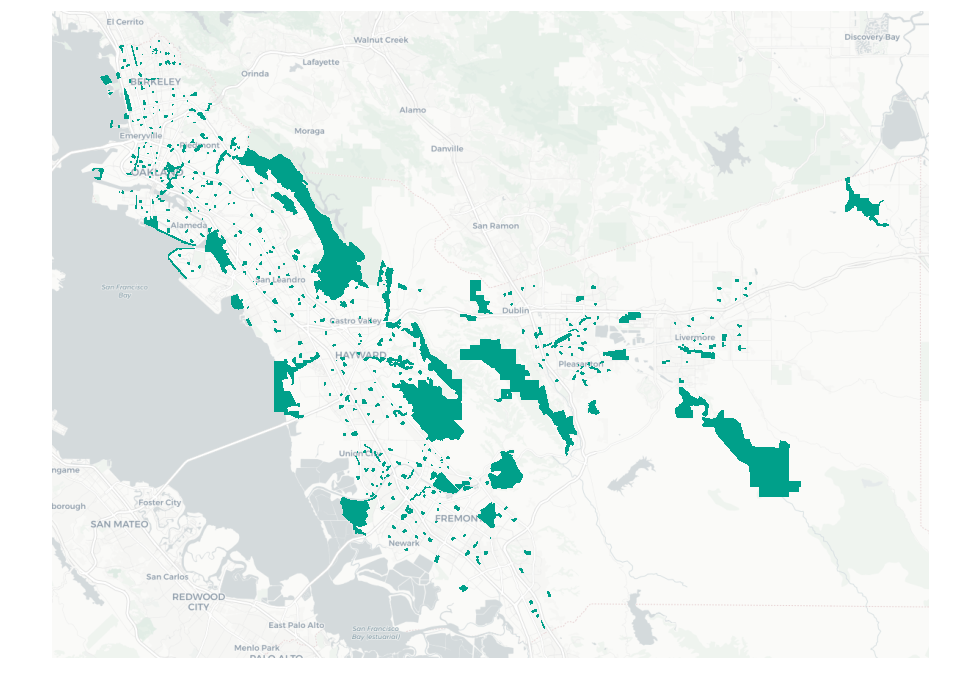
\includegraphics{alameda_destinationchoice_files/figure-latex/parks-map-1.pdf}
\caption{\label{fig:parks-map}Location of parks in Alameda County.}
\end{figure}

We provided the park boundaries layer to a commercial firm, StreetLight Data
Inc., which develops and resells origin-destination matrices derived from
passive device location data. The provider employs a proprietary data processing
engine (called Route Science) to algorithmically transform observed device
location data points (the provider uses in-vehicle GPS units and mobile device
LBS) over time into contextualized, normalized, and aggregated travel patterns.
From these travel patterns, the Route Science processing algorithms infer likely
home Census block group locations for composite groups of people and converts
raw location data points into trip origin and destination points \citep{Pan2006, Friedrich2010}.

For each park polygon, the firm returned a population-weighted estimate of how
many devices were observed by home location block group over several months in
the period between May 2018 and October 2018. We transformed this table such
that it represented the weighted unique devices traveling between block groups
and parks. We discarded home location block groups outside of Alameda County;
the imputed home locations can be far away from the study area for a small
amount of trips and are unlikely to represent common or repeated park
activities.

Table \ref{tab:park-attributes} presents descriptive statistics
on the 500 parks assembled for this study, grouped according to the
park type as defined on CPAD. A little more than half of the parks have
identified paths, while around 40\% of the identified parks have playgrounds and
sport fields.

\begin{table}

\caption{\label{tab:park-attributes}Park Summary Statistics}
\centering
\begin{tabular}[t]{llllll}
\toprule
\multicolumn{2}{c}{ } & \multicolumn{2}{c}{Local Park (N=441)} & \multicolumn{2}{c}{Recreation Area (N=59)} \\
\cmidrule(l{3pt}r{3pt}){3-4} \cmidrule(l{3pt}r{3pt}){5-6}
  &    & Mean & Std. Dev. & Mean  & Std. Dev. \\
\midrule
Acres &  & 59.8 & 370.5 & 125.6 & 505.1\\
Mobile Devices &  & 1450.0 & 6685.4 & 2659.0 & 6161.0\\
\midrule
 &  & N & \% & N & \%\\
type & Local Park & 441 & 88.2 & 0 & 0.0\\
 & Local Recreation Area & 0 & 0.0 & 57 & 11.4\\
 & State Recreation Area & 0 & 0.0 & 2 & 0.4\\
Access & Open Access & 441 & 88.2 & 59 & 11.8\\
 & No Public Access & 0 & 0.0 & 0 & 0.0\\
 & Restricted Access & 0 & 0.0 & 0 & 0.0\\
Playground & FALSE & 224 & 44.8 & 44 & 8.8\\
 & TRUE & 217 & 43.4 & 15 & 3.0\\
Any Sport Field & FALSE & 276 & 55.2 & 39 & 7.8\\
 & TRUE & 165 & 33.0 & 20 & 4.0\\
Football / Soccer & FALSE & 415 & 83.0 & 51 & 10.2\\
 & TRUE & 26 & 5.2 & 8 & 1.6\\
Baseball & FALSE & 364 & 72.8 & 45 & 9.0\\
 & TRUE & 77 & 15.4 & 14 & 2.8\\
Basketball & FALSE & 341 & 68.2 & 52 & 10.4\\
 & TRUE & 100 & 20.0 & 7 & 1.4\\
Tennis & FALSE & 387 & 77.4 & 53 & 10.6\\
 & TRUE & 54 & 10.8 & 6 & 1.2\\
Volleyball & FALSE & 434 & 86.8 & 57 & 11.4\\
 & TRUE & 7 & 1.4 & 2 & 0.4\\
Trail & FALSE & 155 & 31.0 & 22 & 4.4\\
 & TRUE & 286 & 57.2 & 37 & 7.4\\
\bottomrule
\end{tabular}
\end{table}

In order to understand the demographic makeup of the home block groups and
potentially the characteristics of the people who make each trip, we obtained
2013-2017 five-year data aggregations from the American Community Survey
using the \texttt{tidycensus} \citep{Walker2019} interface to the
Census API for several key demographic and built environment variables: the
share of individuals by race, the share of households by income level,
household median income, the share of households with children under 6 years old,
and the household density. An important attribute of
the choice model is the distance from the home block group to the park boundary.
Because we have no information on where in the block group a home is actually
located, we use the population-weighted block group centroid published by the
Census Bureau as the location for all homes in the block group. We then measured
the network-based distance between the park and the home block group centroid
using a walk network derived from OpenStreetMap using the \texttt{networkx} package
for Python \citep{networkx},

\begin{table}

\caption{\label{tab:acs-table}Block Group Summary Statistics}
\centering
\begin{tabular}[t]{>{\raggedright\arraybackslash}p{3cm}rrrrrrr}
\toprule
  & Unique (\#) & Missing (\%) & Mean & SD & Min & Median & Max\\
\midrule
Density: Households per square kilometer & 1041 & 0 & 1709.6 & 1527.8 & 0.0 & 1350.1 & 19490.0\\
Income: Median tract income & 971 & 3 & 93246.3 & 44900.3 & 9821.0 & 85673.0 & 250001.0\\
Low Income: Share of households making less than \$35k & 980 & 0 & 18.4 & 14.0 & 0.0 & 15.1 & 91.7\\
High Income: Share of households making more than \$125k & 1005 & 0 & 32.5 & 20.3 & 0.0 & 30.4 & 100.0\\
Children: Share of households with children under 6 & 985 & 0 & 15.1 & 9.0 & 0.0 & 14.0 & 62.7\\
Black: Share of population who is Black & 929 & 0 & 12.2 & 14.3 & 0.0 & 6.7 & 81.4\\
Asian: Share of population who is Asian & 1011 & 0 & 26.0 & 20.4 & 0.0 & 20.8 & 90.4\\
Other: Share of population who belong to other minority groups & 615 & 0 & 1.5 & 2.4 & 0.0 & 0.5 & 19.6\\
\bottomrule
\end{tabular}
\end{table}

\hypertarget{model}{%
\subsection{Model}\label{model}}

In random utility choice theory, if an individual living in block group \(n\)
wishes to make a park trip, the probability that the individual will choose
park \(i\) from the set of all parks \(J\) can be described as a ratio of the
park's measurable utility \(V_{ni}\) to the sum of the utilities for all parks
in the set. In the common destination choice framework we apply a
multinomial logit model \citep[\citet{Recker1978}]{McFadden1974},
\begin{equation}\label{eq:p}
   P_{ni} = \frac{\exp(V_{ni})}{\sum_{j \in J}\exp(V_{nj})}
\end{equation}
where the measurable utility \(V_{ni}\) is a linear-in-parameters function of
the destination attributes.
\begin{equation}\label{eq:V}
V_{ni} = X\beta
\end{equation}
where \(\beta\) is a vector of estimable coefficients giving the relative utility
(or disutility) of that attribute to the choice maker, all else equal. It is
possible to add amenities of the park or the journey to the utility
equation. However, as the number of alternatives is large, it is impractical to
consider alternative-specific constants or coefficients and therefore not
possible to include attributes of the home block group or traveler \(n\) directly.
We can, however, segment the data and estimate different distance and size
parameters for different segments to observe heterogeneity in the utility
parameters between different socioeconomic groups.

The logarithm of the sum in the denominator of Equation \ref{eq:p} (called the
logsum) provides a measure of the consumer surplus of the choice set
\citep{Williams1977a},
\begin{equation}
CS_n = \ln{{\sum_{j \in J}\exp(V_{nj})}} + C
  \label{eq:logsum}
\end{equation}

where \(C\) is a constant indicating an unknown absolute value. But comparing the
relative logsum values across choice makers, \(CS_n - CS_{n-1}\) gives an
indication of which choice maker has a more valuable choice set. Or, in this
case of a park destination choice model, which choice maker has better access to
parks. Such a ``utility-based'' accessibility term is thus continuously defined,
dervied directly from choice theory, and can contain multiple dimensions of the
attributes of the choice \citep{Handy1997, Dong2006}.

In the most typical cases, researchers estimate the utility coefficients for
destination choice models from household travel surveys. As we have no knowledge
of an appropriate survey on park access, we need to synthesize a suitable
estimation data set. We do this by sampling
\ensuremath{2\times 10^{4}} random discrete device origin-destination pairs from the commercial
passive data matrix, weighted by the volume of the flows. This corresponds to a
4.3\% sample of all the observed device
origin-destination pairs.

The sampled origin-destination pair gives the home location as well as the
``chosen'' alternative for a synthetic person. In principle the individual's
choice set contains all the parks in our dataset; in practice it can be
difficult to estimate choice models with so many alternatives
(\(|J| = 500\)). For this reason we randomly sample 10 additional parks
to serve as the non-chosen alternatives for our synthetic choice maker. Such
random sampling of alternatives reduces the efficiency of the estimated
coefficients but the coefficients remain unbiased \citep{train2009}. As the model has
no alternative-specific constants, the standard likelihood comparison statistic
against the market shares model \(\rho^2\) is not computable. We instead use the
likelihood comparison against the equal shares model \(\rho_0^2\).

The resulting analysis dataset therefore contains \ensuremath{2\times 10^{4}} choice makers that
select between 11 parks including the park they were observed to
choose; the measured distance between the choice maker's block group and all
parks in the choice set; and the acreage of each park in the choice set. We hold
out a random sample of approximately 20\% of choice makers for validation
purposes. We use the \texttt{mlogit} package for R \citep{mlogit, R} to estimate the
multinomial logit models.

\hypertarget{results}{%
\section{Results}\label{results}}

We estimated multinomial logit park activity location choice models including
coefficients for the distance between the park and the home block group and the
acreage of the park. We applied a Yeo-Johnson transformation \citep{Yeo2000} to both
distance and acreage; the Yeo-Johnson transformation replicates the constant
marginal elasticity of a logarithmic transformation while avoiding undefined
values (\(YJ(0) = 0\)). For simplicity, we call this transformation \texttt{log()} in the
model results tables. Using a constant marginal elasticity is better reflective
of how people perceive distances and sizes; a one-mile increase to a trip
distance is more impactful to a one-mile trip than a ten-mile trip.

Table \ref{tab:base-modelsummary} presents the model estimation results for a
series of models with different utility function definitions, each estimated on the
complete set of synthetic choice makers. The first model --- named ``Network
Distance'' --- only considers the distance to the park and the size of the park
in the utility equation. The estimated coefficients are significant and of the
expected sign: That is, individuals will travel further distances to reach larger
parks. The ratio of the estimated coefficients implies that on average, people
will travel 3.3089752 times further to reach a park twice as large.

The second and third models in Table \ref{tab:base-modelsummary} include a
vector of park attributes. In the model labeled ``Park Attributes,'' the presence
of any sport field is considered with a single dummy value, and in the ``Sport
Detail'' model this variable is disaggregated into facilities for different
sports. The value of the size and distance coefficients change modestly from
the ``Network Distance'' model, with the implied size to distance trade-off rising
to 3.3089752. Examining the two amenities models --- independently and in
comparison with each other --- reveals a few surprising findings. First, it
appears that playgrounds and sport fields in general contribute \emph{negatively} to
the choice utility equation. This is both unintuitive and contradictory to
previous findings in this space \citep[e.g.,][]{Kinnell2006}. Considering different
sports separately, there is a wide variety of observed response with tennis and
volleyball facilities attracting more trips, and football and basketball
facilities attracting fewer, all else equal. Trails and walking paths give
substantive positive utility in both models. The difference in likelihood statistics
between the three models is significant (likelihood ratio test
\(p\)-value \ensuremath{3.5989633\times 10^{-4}}), and so in spite of the curious aggregate findings,
we move forward with this utility specification.

\begin{table}

\caption{\label{tab:base-modelsummary}Estimated Model Coefficients}
\centering
\begin{tabular}[t]{lccc}
\toprule
  & Network Distance & Park Attributes & Sport Detail\\
\midrule
log(Distance) & -1.354*** & -1.394*** & -1.390***\\
 & (0.022) & (0.022) & (0.022)\\
log(Acres) & 0.409*** & 0.353*** & 0.348***\\
 & (0.011) & (0.012) & (0.012)\\
Playground &  & -0.437*** & -0.551***\\
 &  & (0.049) & (0.049)\\
Trail &  & 0.555*** & 0.563***\\
 &  & (0.052) & (0.053)\\
Sport Field &  & -0.324*** & \\
 &  & (0.050) & \\
Basketball &  &  & -0.237***\\
 &  &  & (0.068)\\
Baseball &  &  & 0.075\\
 &  &  & (0.067)\\
Football / Soccer &  &  & -0.490***\\
 &  &  & (0.095)\\
Tennis &  &  & 0.231***\\
 &  &  & (0.066)\\
Volleyball &  &  & 0.607***\\
 &  &  & (0.135)\\
Other Sport &  &  & -0.150*\\
 &  &  & (0.087)\\
\midrule
Num.Obs. & 3971 & 3971 & 3971\\
AIC & 11600.2 & 11306.5 & 11293.6\\
Log.Lik. & -5798.103 & -5648.236 & -5636.809\\
rho2 &  &  & \\
rho20 & 0.391 & 0.407 & 0.408\\
\bottomrule
\multicolumn{4}{l}{\textsuperscript{} * p < 0.1, ** p < 0.05, *** p < 0.01}\\
\end{tabular}
\end{table}

It is worth investigating the heterogeneity in preferences that exist among
different demographic groups. Though the income and ethnicity of the synthetic
park visitors is not known, we can segment the estimation dataset based on the
socioeconomic makeup of the visitors' residence block group. The models presented in
Table \ref{tab:grouped-modelsummary} were
estimated on segments developed in this manner.
Models under the ``Minority'' heading include a
race-based segmentation: simulated individuals living in block groups with more
than thirty percent Black persons are included in the ``\textgreater30\% Black'' model, an
analogous segmentation for block groups with high Asian populations are in the
``\textgreater30\% Asian'' model, and the ``Other'' model contains all other block groups.
Another set of model segmentation relies on the share of the population in each
block group with household incomes above or below certain thresholds. Again,
we use the threshold definitions based on in \ref{tab:acs-table}.

\begin{landscape}\begin{table}

\caption{\label{tab:grouped-modelsummary}Estimated Model Coefficients with Block Group Segmentations}
\centering
\resizebox{\linewidth}{!}{
\begin{tabular}[t]{lccccccccc}
\toprule
\multicolumn{1}{c}{ } & \multicolumn{3}{c}{Minority} & \multicolumn{3}{c}{Income} & \multicolumn{3}{c}{Children} \\
\cmidrule(l{3pt}r{3pt}){2-4} \cmidrule(l{3pt}r{3pt}){5-7} \cmidrule(l{3pt}r{3pt}){8-10}
  & > 30\% Asian & > 30\% Black & Other & > 30\% Low income & > 50\% High income & Other  & > 25\% children & < 5\% children & Other  \\
\midrule
\cellcolor{gray!6}{log(Distance)} & \cellcolor{gray!6}{-1.328***} & \cellcolor{gray!6}{-1.522***} & \cellcolor{gray!6}{-1.377***} & \cellcolor{gray!6}{-1.419***} & \cellcolor{gray!6}{-1.309***} & \cellcolor{gray!6}{-1.394***} & \cellcolor{gray!6}{-1.236***} & \cellcolor{gray!6}{-1.594***} & \cellcolor{gray!6}{-1.398***}\\
 & (0.038) & (0.064) & (0.031) & (0.051) & (0.051) & (0.029) & (0.059) & (0.083) & (0.026)\\
\cellcolor{gray!6}{log(Acres)} & \cellcolor{gray!6}{0.373***} & \cellcolor{gray!6}{0.305***} & \cellcolor{gray!6}{0.343***} & \cellcolor{gray!6}{0.338***} & \cellcolor{gray!6}{0.342***} & \cellcolor{gray!6}{0.354***} & \cellcolor{gray!6}{0.313***} & \cellcolor{gray!6}{0.372***} & \cellcolor{gray!6}{0.356***}\\
 & (0.020) & (0.033) & (0.017) & (0.027) & (0.028) & (0.015) & (0.030) & (0.044) & (0.014)\\
\cellcolor{gray!6}{Playground} & \cellcolor{gray!6}{-0.520***} & \cellcolor{gray!6}{-0.395***} & \cellcolor{gray!6}{-0.628***} & \cellcolor{gray!6}{-0.515***} & \cellcolor{gray!6}{-0.499***} & \cellcolor{gray!6}{-0.585***} & \cellcolor{gray!6}{-0.431***} & \cellcolor{gray!6}{-0.879***} & \cellcolor{gray!6}{-0.540***}\\
 & (0.085) & (0.122) & (0.070) & (0.104) & (0.123) & (0.063) & (0.124) & (0.180) & (0.057)\\
\cellcolor{gray!6}{Trail} & \cellcolor{gray!6}{0.658***} & \cellcolor{gray!6}{0.361***} & \cellcolor{gray!6}{0.638***} & \cellcolor{gray!6}{0.306***} & \cellcolor{gray!6}{0.896***} & \cellcolor{gray!6}{0.612***} & \cellcolor{gray!6}{0.122} & \cellcolor{gray!6}{0.744***} & \cellcolor{gray!6}{0.638***}\\
 & (0.095) & (0.128) & (0.076) & (0.109) & (0.148) & (0.068) & (0.126) & (0.190) & (0.062)\\
\cellcolor{gray!6}{Basketball} & \cellcolor{gray!6}{-0.011} & \cellcolor{gray!6}{-0.357*} & \cellcolor{gray!6}{-0.422***} & \cellcolor{gray!6}{-0.187} & \cellcolor{gray!6}{-0.109} & \cellcolor{gray!6}{-0.300***} & \cellcolor{gray!6}{-0.316*} & \cellcolor{gray!6}{-0.301} & \cellcolor{gray!6}{-0.215***}\\
 & (0.109) & (0.184) & (0.102) & (0.153) & (0.160) & (0.088) & (0.172) & (0.262) & (0.078)\\
\cellcolor{gray!6}{Baseball} & \cellcolor{gray!6}{0.130} & \cellcolor{gray!6}{0.192} & \cellcolor{gray!6}{-0.012} & \cellcolor{gray!6}{0.054} & \cellcolor{gray!6}{-0.108} & \cellcolor{gray!6}{0.139} & \cellcolor{gray!6}{0.127} & \cellcolor{gray!6}{-0.038} & \cellcolor{gray!6}{0.085}\\
 & (0.112) & (0.172) & (0.097) & (0.145) & (0.165) & (0.085) & (0.168) & (0.256) & (0.076)\\
\cellcolor{gray!6}{Football / Soccer} & \cellcolor{gray!6}{-0.479***} & \cellcolor{gray!6}{-1.068***} & \cellcolor{gray!6}{-0.359***} & \cellcolor{gray!6}{-0.886***} & \cellcolor{gray!6}{-0.263} & \cellcolor{gray!6}{-0.451***} & \cellcolor{gray!6}{-0.163} & \cellcolor{gray!6}{-0.964***} & \cellcolor{gray!6}{-0.538***}\\
 & (0.153) & (0.283) & (0.137) & (0.226) & (0.223) & (0.120) & (0.228) & (0.357) & (0.110)\\
\cellcolor{gray!6}{Tennis} & \cellcolor{gray!6}{0.386***} & \cellcolor{gray!6}{-0.535**} & \cellcolor{gray!6}{0.315***} & \cellcolor{gray!6}{-0.096} & \cellcolor{gray!6}{0.659***} & \cellcolor{gray!6}{0.201**} & \cellcolor{gray!6}{0.348**} & \cellcolor{gray!6}{-0.059} & \cellcolor{gray!6}{0.229***}\\
 & (0.108) & (0.210) & (0.095) & (0.163) & (0.146) & (0.085) & (0.163) & (0.264) & (0.076)\\
\cellcolor{gray!6}{Volleyball} & \cellcolor{gray!6}{0.703***} & \cellcolor{gray!6}{-0.077} & \cellcolor{gray!6}{0.452**} & \cellcolor{gray!6}{0.433} & \cellcolor{gray!6}{0.446*} & \cellcolor{gray!6}{0.593***} & \cellcolor{gray!6}{0.549*} & \cellcolor{gray!6}{0.424} & \cellcolor{gray!6}{0.610***}\\
 & (0.197) & (0.615) & (0.212) & (0.403) & (0.257) & (0.177) & (0.329) & (0.538) & (0.154)\\
\cellcolor{gray!6}{Other Sport} & \cellcolor{gray!6}{-0.051} & \cellcolor{gray!6}{-0.258} & \cellcolor{gray!6}{-0.212*} & \cellcolor{gray!6}{-0.495**} & \cellcolor{gray!6}{0.010} & \cellcolor{gray!6}{-0.133} & \cellcolor{gray!6}{0.268} & \cellcolor{gray!6}{-0.417} & \cellcolor{gray!6}{-0.223**}\\
 & (0.141) & (0.252) & (0.126) & (0.222) & (0.184) & (0.112) & (0.212) & (0.334) & (0.100)\\
\midrule
\cellcolor{gray!6}{Num.Obs.} & \cellcolor{gray!6}{1365} & \cellcolor{gray!6}{579} & \cellcolor{gray!6}{2027} & \cellcolor{gray!6}{777} & \cellcolor{gray!6}{758} & \cellcolor{gray!6}{2436} & \cellcolor{gray!6}{544} & \cellcolor{gray!6}{358} & \cellcolor{gray!6}{3069}\\
AIC & 3939.0 & 1739.9 & 5561.4 & 2396.3 & 1908.9 & 6975.0 & 1810.6 & 895.4 & 8574.4\\
\cellcolor{gray!6}{Log.Lik.} & \cellcolor{gray!6}{-1959.519} & \cellcolor{gray!6}{-859.966} & \cellcolor{gray!6}{-2770.689} & \cellcolor{gray!6}{-1188.142} & \cellcolor{gray!6}{-944.432} & \cellcolor{gray!6}{-3477.497} & \cellcolor{gray!6}{-895.280} & \cellcolor{gray!6}{-437.678} & \cellcolor{gray!6}{-4277.200}\\
rho2 &  &  &  &  &  &  &  &  & \\
\cellcolor{gray!6}{rho20} & \cellcolor{gray!6}{0.401} & \cellcolor{gray!6}{0.381} & \cellcolor{gray!6}{0.430} & \cellcolor{gray!6}{0.362} & \cellcolor{gray!6}{0.480} & \cellcolor{gray!6}{0.405} & \cellcolor{gray!6}{0.314} & \cellcolor{gray!6}{0.490} & \cellcolor{gray!6}{0.419}\\
\bottomrule
\multicolumn{10}{l}{\textsuperscript{} * p < 0.1, ** p < 0.05, *** p < 0.01}\\
\end{tabular}}
\end{table}
\end{landscape}

The model estimates in Table \ref{tab:grouped-modelsummary} reveal that there
is noticeable heterogeneity in the response among different socioeconomic
groups. Park visitors living in block groups with a high proportion of Black and
low-income residents show less affinity for trails and other walkways, but
appear are also considerably to be more sensitive to the distance of a park.
Visitors living in high-income neighborhoods are more attracted to the amenities
of a park, or rather these visitors do not show significant negative
coefficients for amenities, e.g.~basketball courts and football fields.

Seeing that there is a difference in the response in the model segmentation,
it is also worth considering the role of our segmentation thresholds in these
findings. Figure \ref{fig:split-plots} shows the estimated coefficients and
confidence intervals for these different amenities at different threshold levels
of segmentation. The threshold level means that at least that percent
of the block group's population falls in that category. The confidence intervals
widen as more observations are excluded from the model. The estimated coefficients
for the different segmentations are identical when the share equals zero, and
simply represent the ``Sport Detail'' model from Table \ref{tab:base-modelsummary}.

Overall, increasing the segmentation threshold level reveals some additional
information about user preferences. First, it should be noted that there is
some inconsistency: for instance, block groups with at least 40\% of low income
households show a lower importance of distance than block groups with either
30\% or 50\% low income households. The increasing width of the confidence interval,
however, means it is difficult to make generalized statements. Residents of
block groups with a higher share of Asian or high income households both show
relatively more affinity for tennis courts and trails. Block groups with high
Black populations show a somewhat greater preference for playgrounds, as well
appearing to be the most distance-sensitive group.

\begin{figure}
\centering
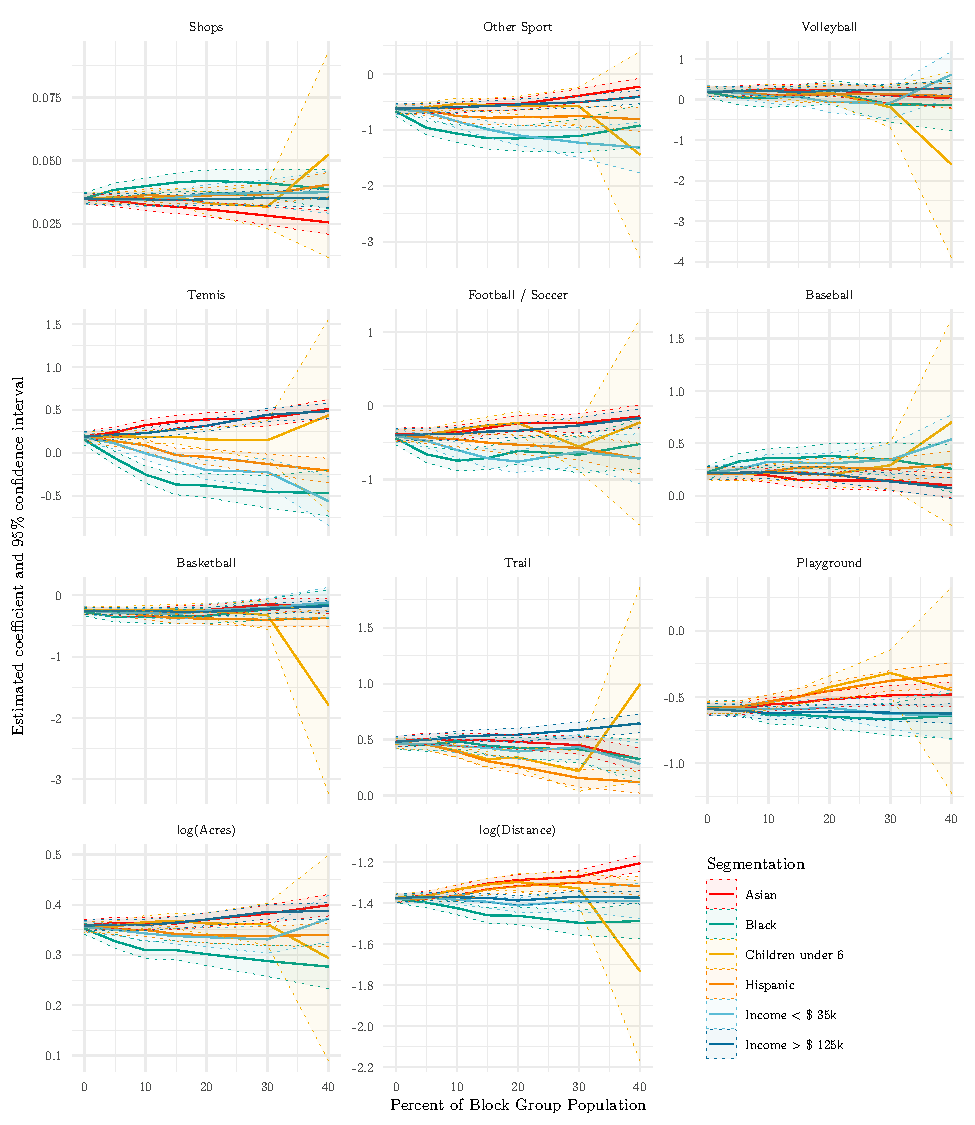
\includegraphics{alameda_destinationchoice_files/figure-latex/split-plots-1.pdf}
\caption{\label{fig:split-plots}Estimated utility coefficients and 95\% confidence intervals for park amenities at different socioeconomic threshold levels.}
\end{figure}

\hypertarget{model-application-equity-analysis-of-covid-19-street-openings}{%
\subsection{Model Application: Equity Analysis of COVID-19 Street Openings}\label{model-application-equity-analysis-of-covid-19-street-openings}}

In spring and summer 2020, cities across the world responded to the COVID-19
pandemic by converting city streets into temporary pedestrian plazas. The stated
goals of this policy included providing recreational space that would allow
people to walk and exercise outside with sufficient personal space and less risk
of conflict from vehicle traffic. This policy created several dozen temporary
open spaces in urbanized areas of the county. In this section, we apply the
models estimated above to evaluate the benefits of this policy in terms of
aggregate value, as well as the equity of the policy with respect to different
income and ethnic groups.

We obtained the list of streets in Alameda County that were reported closed
in the ``Shifting Streets'' COVID-19 mobility dataset \citep{slowstreets}. This dataset
reports that 74 individual streets were closed to vehicle
traffic (and thereby opened as public spaces); these streets represent
27.5730459 total miles across the cities
of Berkeley, Oakland, and Alameda. For the purposes of this analysis, we
represent each opened street as a single ``park'' without any sport facilities or
playgrounds, but with a trail / walking path. The database provides the opened
streets as polyline objects; we assert a 25-foot buffer around the line to
represent a polygon with a measurable area. Finally, we measure the network-based
distance from each population-weighted block group centroid to the nearest
boundary of each new open space facility created by this policy.

Using this new dataset --- augmented with parks added by street openings --- we
applied the ``Sport Detail'' non-segmented model to calculate park choice utilities
and utility-based accessibility values for each block group in Alameda County.
As shown with Equation \eqref{eq:logsum}, the difference in utility-based
accessibility values with and without the opened streets is the consumer
surplus provided by the policy. This surplus is given in a unitless utility,
but it is possible to convert the surplus into monetary units by diving the
surplus by a cost utility coefficient. The dataset used for this research does
not have any information on travel costs or entrance fees, and such data would
likely not be relevant in the context of urban parks. As a result, there is no
direct link between the utility and a monetary cost in our estimated models.

As a substitution, we use an estimate of the cost coefficient obtained from the
open-source activity-based travel demand model ActivitySim, which is itself
based on the regional travel model employed by the Metropolitan
Transportation Commission (MTC), the San Francisco Bay regional MPO.
ActivitySim uses a cost coefficient of
\(-0.6\) divided by the each simulated agent's value of time to determine
destination choices for non-work trips.\footnote{To be precise, this is the cost
  coefficient on the mode choice model for social, recreational, and other trip
  purposes, which influences destination choice through a logsum-based impedance
  term.} In ActivitySim, as in most activity-based travel models, the value of
time is considered to vary with an individual's income, but in this aggregate
destination choice model, an aggregate value of time will suffice. The average
value of time in the synthetic population for the Bay Area is \$7.75
per hour, resulting in a cost coefficient on the destination choice utility of
\(-0.215\). Dividing the difference in accessibility logsums by the negative of
this value gives an initial estimate of the monetary value of the policy
to each park user.

Figure \ref{fig:logsumsmap} presents this monetary valuation spatially.
Unsurprisingly, the benefits are concentrated in the block groups surrounding
the opened streets. Most residents of central Oakland see a benefit of somewhere
around \$1, while some zones see an equivalent benefit of as much as \$30. One
property of logsum-based accessibility terms is that there is some benefit given
for simply having more options, whether or not those options are attractive in
any way. In this application, these benefits are small, on the order of 10 cents
for most block groups away from where the street openings occurred.

\begin{figure}
\centering
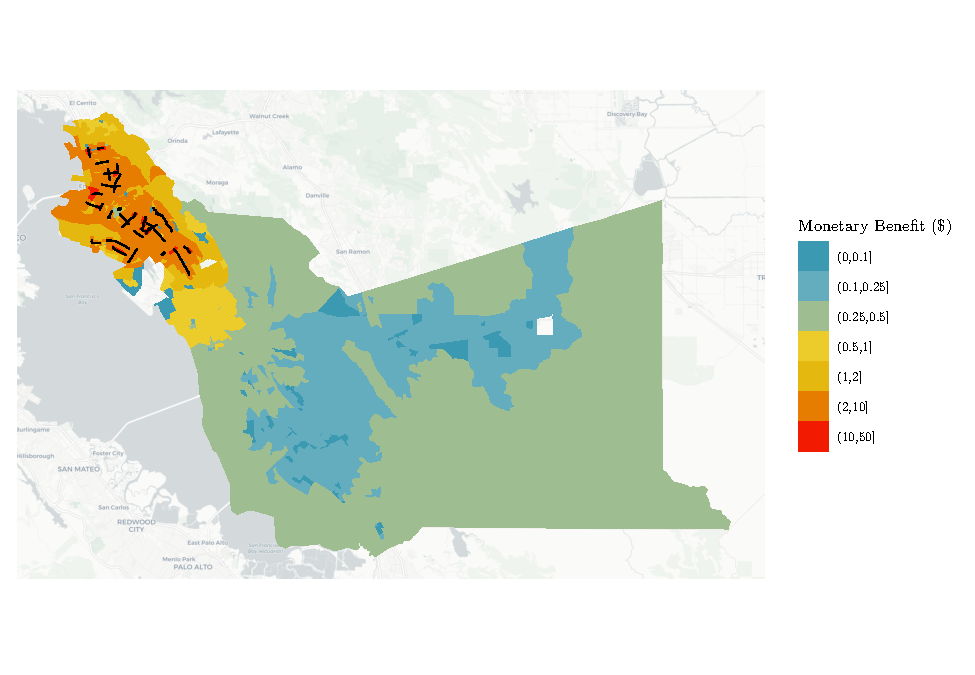
\includegraphics{alameda_destinationchoice_files/figure-latex/logsumsmap-1.pdf}
\caption{\label{fig:logsumsmap}Monetary value of street opening to residents based on utility change.}
\end{figure}

More interesting than the total benefit or even its spatial distribution, however,
is the social equity of its distribution among different population segments.
If we assign the block-group level monetary benefit to each household in the block
group, we can begin to allocate the distribution of benefits proportionally to
households of different sociodemographic classifications. Specifically, if a block
group with \(N\) total households has a measured consumer surplus \(\delta CS\), then the
share of the total benefits going to a particular population segment \(k\) is

\begin{equation}
  S_k = N * P_k * \delta CS
  \label{eq:cs-alloc}
\end{equation}

where and \(P_k\) is the proportion of the block group's population in segment \(k\).
There is some opportunity for confusion when some demographic variables we use
(share of households with children, household income) are defined at the
household level and other (ethnicity) are defined at the person level. It is similarly
not clear whether the benefits of improved park access should be assigned at
the person level, the household level, or the number of total park trip makers in
each block group. For consistency and simplicity, we assert that the benefit is
assigned to each household, and that persons receive a proportional share of the
household benefit. For example, a block group with 30\% Black individuals will
receive 30\% of the benefits assigned to all the households in the block group.

Table \ref{tab:equity} shows the total benefit assigned to households in this way
as well as the share of all monetary benefits in the region. In some cases, the
policy of opening streets as public spaces had a pro-social benefit, as 18.7\%
of benefits went to Black individuals, even though only 11.4\% of the population
of Alameda County is Black. Similarly, roughly one-quarter of total benefits
went to households making less than \$35,000 per year even though only one-fifth
of the households are in this category. On the other hand, a smaller than
expected share of benefits is allocated to Asian individuals and households making
more than \$125,000 per year.

\begin{table}

\caption{\label{tab:equity}Equity Distribution of Street Opening Benefits}
\centering
\begin{tabular}[t]{>{\raggedright\arraybackslash}p{1.8in}>{\centering\arraybackslash}p{0.8in}>{\centering\arraybackslash}p{0.8in}>{\centering\arraybackslash}p{0.8in}>{\centering\arraybackslash}p{0.8in}>{\centering\arraybackslash}p{0.8in}}
\toprule
Group & Benefit & Percent of Benefits & Households & Percent of Households & Difference in Distribution\\
\midrule
Households with Children under 6 & \$91,530 & 14.15 & 86,095 & 15.13 & -0.9828\\
Income < \$35k & \$157,608 & 24.36 & 102,580 & 18.03 & 6.3330\\
Income > \$125k & \$164,211 & 25.38 & 190,573 & 33.49 & -8.1090\\
Black & \$120,749 & 18.66 & 64,929 & 11.41 & 7.2526\\
Asian & \$125,397 & 19.38 & 159,001 & 27.94 & -8.5599\\
\addlinespace
Other & \$9,522 & 1.47 & 7,878 & 1.38 & 0.0874\\
White / Hispanic & \$391,355 & 60.49 & 337,262 & 59.27 & 1.2200\\
All Households & \$647,023 & 100.00 & 569,070 & 100.00 & 0.0000\\
\bottomrule
\end{tabular}
\end{table}

By this analysis, the policy to open streets as pedestrian plazas and public
spaces appears to be a pro-social policy with substantial benefits to the
community. There are some limitations and caveats that ought to be considered;
for example, COVID-19 led to the closure of some park facilities that were not
captured in this analysis. This policy would lead to a decrease in the consumer
surplus for park access, which might overwhelm or at least change the distribution
of benefits we measured here. A policy of permanently closing these streets to
vehicle traffic would also have potentially deleterious effects on
transportation access that would need to be considered against the benefits
we measure here; in the case of the COVID-19 quarantine, the opportunity
cost of closing a street to nonexistent vehicle traffic is basically zero.

\hypertarget{limitations-and-future-directions}{%
\section{Limitations and Future Directions}\label{limitations-and-future-directions}}

The ideal dataset for estimating individual choices would be a high-quality,
large-sample household travel survey of real individuals. Such a survey would
give details on whether an observed trip to a park was actually a recreation
trip or rather a different activity entirely. The individual-level demographic
data would also be valuable in understanding more clearly the observed
heterogeneity in response among different income or ethnic groups. Additionally,
the trends and correlations revealed in the presented models may reflect
situational inequalities rather than true preferences. For example, the
distinct observed parameters on size and distance for minority block groups may
indicate that areas with large minority populations tend to have smaller parks
that are more geographically distributed relative to other regions of the region.
Transit access may also affect park choice and how far people are willing to
travel to access a park. Preliminary analysis of our source data indicates a
qualitative correlation between good transit access and diverse park use from
both a geographic and demographic perspective.

We limited our analysis to home locations and parks in Alameda County,
California. It is possible that some Alameda residents visit parks in
neighboring counties, just as it is possible that parks in Alameda County
attract trips from outside the county borders. This is most likely for block
groups and parks on the north and south borders of the county. The lower
measured accessibility in the area around Berkeley in the northern part of the
county () is likely affected by the ommission of parks and residents in Contra
Costa County.

Using Euclidean distance to represent the distance between the block group
centroid and the border of the park leaves something to be desired: Depending on
network topography and built environment characteristics, there may be a
significant variation in perceived travel times between two parks with similar
straight-line distances. That said, a more precise network-based measure might
not overcome the inaccuracies resulting from our necessarily measuring distances
from the block group centroid. As above, an individual-level survey where the
home location is explicitly known would be preferable regardless of the distance
method employed.

The activity location data used in this specific analysis treats all days of the
week and day periods together; it is likely that weekend park choice is
substantially different from weekday choice, as the activities performed may be
the same. Also recall that the data consider each device-park pair as a unique
trip. Repeated trips to the same park may not be properly considered in the data
sample. A more precise time-of-day and day-of-week segmentation is warranted.

We applied a naive random sampling of the alternatives in our model estimation
and validation; a more considered approach involving hierarchical destination
sampling may yield more efficient estimates and therefore a clearer picture of
the role of size, distance, and other amenities on the observed choices. The
relatively weak predictive power of such a simple model formulation (size and
distance only) indicates that there is potential to examine the role that
additional park amenities --- ball fields, playgrounds, water features, etc. ---
play in the relative attractiveness of parks for different market segments. The
quality of park maintenance is another important feature identified in the
recreation literature \citep{Fletcher2003} that is not included here.

\hypertarget{conclusions}{%
\section{Conclusions}\label{conclusions}}

As transportation professionals seek to improve access to parks and better
coordinate transportation and land use efforts --- and as researchers more
generally try to understand the role parks and open spaces play in public health
and society --- it is increasingly important to better understand how, when, and
why individuals travel to parks. This intersection between recreation and
transportation has received relatively little exploration, partially because
travel survey data emphasizes weekday travel and because the role of parks in
daily activities can be more complicated than with other land uses. This study
contributes to the understanding of recreation access by presenting a method to
develop access measures explicitly based on the observed choices of individuals.
The resulting access measure is continuously defined and incorporates multiple
dimensions of access, including the travel necessary to reach all nearby parks
as well as the amenities of each of those parks. Further, the measure we have
presented reveals heterogeneous preferences for travel and park size across
market segments, a heterogeneity that could perhaps be incorporated into an
understanding of accessibility.

With the growing availability of passive transportation data, there is a
correspondingly increased opportunity to explore such data to develop a better
understanding of travel patterns in more careful detail than is possible with
household travel surveys. Capturing a sufficiently large survey to study trip
patterns to a single park is an enormous undertaking, and doing such an exercise
for an entire park system is prohibitively expensive and time-consuming. Passive
data sets therefore enable analyses that would be unlikely or impossible by
other means. Challenges to the representativeness and comprehensiveness of
passive data products are in many cases fair, but this should not preclude their
use in cases where traditional techniques are not practicable.

\hypertarget{acknowledgments}{%
\section*{Acknowledgments}\label{acknowledgments}}
\addcontentsline{toc}{section}{Acknowledgments}

Graphics and tables were developed using several open-source R packages
\citep{ggmap, modelsummary, wesanderson}.

\bibliography{book.bib}


\end{document}


